\documentclass{standalone}

\usepackage{tikz}

\begin{document}
\Large
\begin{tikzpicture}
% \draw[help lines, black!30] (0,0) grid (12,12);
\foreach \a in 
    {(2,2),(2,6)}
    {\node at \a {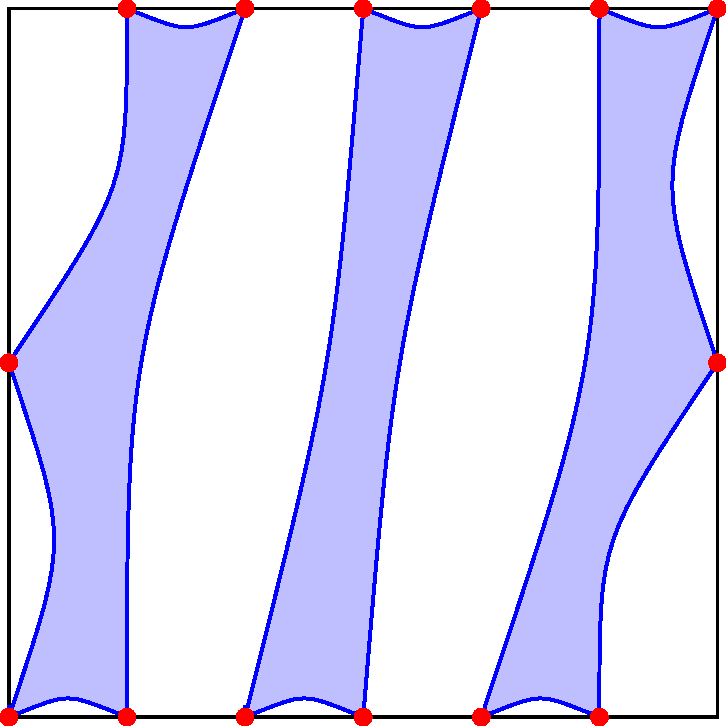
\includegraphics[width=4.1cm]{constr3clear.pdf}};};
\foreach \a in 
    {(6,0), (6,4)}
    {\draw[line width=0.5mm, black!50] \a rectangle ++(4,4);
    \fill 
        \a++(1,2) circle (0.25)
        \a++(2,2) circle (0.25)
        \a++(3,2) circle (0.25);
        };
\foreach \a in 
    {(6,0)}
    {\draw[line width=0.7mm]
        \a++(1,2) -- ++(0,4)
        \a++(1,2) -- ++(1,4)
        \a++(2,2) -- ++(0,4)
        \a++(2,2) -- ++(1,4)
        \a++(3,2) -- ++(0,4);
    };
\end{tikzpicture}
\end{document}